% f2015hbw_q20_pyramid.tex — 2015 年高考数学·湖北卷·文科 第 20 题（阳马）
%
% 【来源】`.work/phase3-b20/source/2015湖北文.pdf`（SHA-256
%   801e73338b6c4c747cc76b14e167d590a34e0b5a13a47719e5ee6cd4337e4cd2），
%   第 2 页（合订本页 954）；内容对象 34。逐路径实测见
%   `.work/phase3-b20/figure-inventory.md`。
%
% 【坐标口径】源 PDF 用户空间（原点左下、y 向上）。本图本地坐标
%   (x, y) = (x_page − 279.213, y_page − 191.72)，1 单位 = 1 TeX pt。
%   路径坐标逐点照录内容流（含三次贝塞尔控制点）。
%
% 元素计数：11 条路径（6 实＋5 虚）＋6 个标签
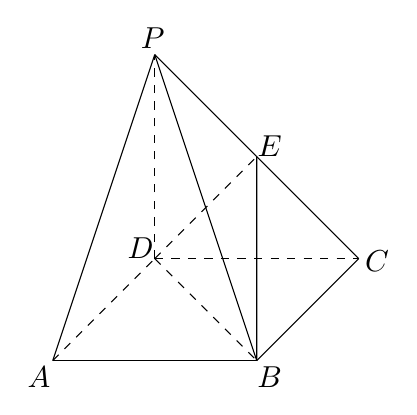
\begin{tikzpicture}[x=1pt, y=1pt,
    every node/.style={inner sep=0pt, font=\fontsize{10.5pt}{12.6pt}\selectfont}]
  \draw[line width=0.3985pt] (0.0000,0.0000)   (0.0000,0.0000)   -- (73.7162,0.0000);
  \draw[line width=0.3985pt] (73.7162,0.0000)   (73.7162,0.0000)   -- (110.5688,36.8525);
  \draw[line width=0.3985pt] (36.8525,110.5688)   (36.8525,110.5688)   -- (0.0000,0.0000);
  \draw[line width=0.3985pt] (36.8525,110.5688)   (36.8525,110.5688)   -- (73.7162,0.0000);
  \draw[line width=0.3985pt] (36.8525,110.5688)   (36.8525,110.5688)   -- (110.5688,36.8525);
  \draw[line width=0.3985pt] (73.7162,0.0000)   (73.7162,0.0000)   -- (73.7105,73.7105);
  \draw[line width=0.3985pt, dash pattern=on 2.98883pt off 2.98883pt, dash phase=0.0pt] (0.0000,0.0000)   (0.0000,0.0000)   -- (36.8525,36.8525);
  \draw[line width=0.3985pt, dash pattern=on 2.98883pt off 2.98883pt, dash phase=0.0pt] (36.8525,36.8525)   (36.8525,36.8525)   -- (110.5688,36.8525);
  \draw[line width=0.3985pt, dash pattern=on 2.98883pt off 2.98883pt, dash phase=0.0pt] (36.8525,36.8525)   (36.8525,36.8525)   -- (36.8525,110.5688);
  \draw[line width=0.3985pt, dash pattern=on 2.98883pt off 2.98883pt, dash phase=0.0pt] (36.8525,36.8525)   (36.8525,36.8525)   -- (73.7105,73.7105);
  \draw[line width=0.3985pt, dash pattern=on 2.98883pt off 2.98883pt, dash phase=0.0pt] (36.8525,36.8525)   (36.8525,36.8525)   -- (73.7162,0.0000);

  \node[anchor=center] at (36.137,116.570) {$P$};  % 源中心 (315.35,308.29)
  \node[anchor=center] at (78.337,77.670) {$E$};  % 源中心 (357.55,269.39)
  \node[anchor=center] at (31.737,40.820) {$D$};  % 源中心 (310.95,232.54)
  \node[anchor=center] at (-4.963,-5.880) {$A$};  % 源中心 (274.25,185.84)
  \node[anchor=center] at (117.137,35.920) {$C$};  % 源中心 (396.35,227.64)
  \node[anchor=center] at (78.387,-5.880) {$B$};  % 源中心 (357.60,185.84)

\end{tikzpicture}
%
% 【自验结果】
%   探针：latexmk -pdfxe（待跑）。
